\documentclass[12pt,doublespacing]{article}

\usepackage{amsmath}
\usepackage{graphicx}
\usepackage{amssymb}
\usepackage{natbib}
\usepackage[T1]{fontenc}        %for danish letters
\usepackage[latin1]{inputenc}   %for danish letters
%\usepackage{rotating}



%\usepackage[left,pagewise]{lineno}
\usepackage[left,running]{lineno}

%\usepackage{doublespace}
\usepackage{setspace}

%\newcommand{\tablenotemark}[1]{${}^{#1}$}
%\newcommand{\tablenotetext}[2]{${}^{#1}${#2}}

\usepackage{caption2}
%%%%%%%%%%%%new table captions%%%%%%%%%%%%%%%%%%%%%%%%%%%%%%%%%%%%%
%\newcommand{\tabcap}[1]{\onelinecaptionsfalse\captionstyle{flushleft}\renewcommand{\captionfont}{\bfseries}\renewcommand{\captionlabelfont}{\hspace{0.125cm}\bfseries}\caption{#1}}
\newcommand{\tabcap}[1]{\onelinecaptionsfalse\captionstyle{flushleft}{\hspace{0.125cm}}\caption{#1}}
%%%%%%%%%%%%%%%%%%%%%%%%%%%%%%%%%%%%%%%%%%%%%%%%%%%%%%%%%%%%%%%%%%%%%

\doublespace


\begin{document}

\linenumbers


\title{Evaluation of the Hooghoudt drainage equation}


\author{Mikkel Mollerup$^{1}\thanks{Corresponding author}$ \and S�ren Hansen$^{2}$ \and Per Abrahamsen$^{2}$ \and Carsten Petersen$^{2}$}

\maketitle

\noindent $^{1}$Department of Basic Sciences and Environment,
Faculty of Life Sciences \\ University of
Copenhagen, Denmark, mmo@life.ku.dk\\
\\
\noindent $^{2}$Department of Basic Sciences and Environment,
Faculty of Life Sciences \\ University of
Copenhagen, Denmark\\


\begin{abstract}
Hooghoudt blabre blabre
\end{abstract}


%%\begin{article}

\section{Introduction}
Hooghoudt blabre blabre

%% ------------------------------------------------------------------------ %%
%
%  SECTION HEADS
%
%% ------------------------------------------------------------------------ %%


The model applied in the present studies, DAISY
\citep{Hansen,Abrahamsen} is used for describing the crop
production as well as water and nitrogen balances in the root zone.

DAISY have in numerous studies
\citep[e.g.][]{Styczen2,Refsgaard,Thorsen,Boegh,HansenRolmer,vanderKeur}
been applied for estimation of water balances or simulation of
pollution of non-point sources arising from agricultural production on
a catchment scale. In many of the studies the processes in the root
zone are handled by a described 1D with DAISY whereas the
hydrological catchment model MIKE SHE \citep{Abbott} has been
applied for 2D modelling of the surface flow and 3D modelling of the
groundwater
flow.\\

Common for all the mentioned studies is that they required a very
large number of DAISY simulations due to different soil, crop
,management, etc within the catchment. Thus a fast computation of
the processes in the unsaturated zone is crucial. For agricultural
fields with parallel placed pipe drains the flow towards the drains is a
two dimensionally process. In the 1D DAISY is the estimation of the
drain fluxes based on the theory by Hooghoudt which assumes
steady state conditions (and?). DAISY has recently been developed
so the model also can be used for 2D simulations with a more
precise calculation of drain fluxes. But compared with 1D simulation,
2D (or 3D) simulations of water and solute movement in the
unsaturated zone are from a computational point of view very
expensive.\\

The question is, can the 2D drain simulations with adequate
precision be replaced by 1D simulations for estimation of water and
solute drain fluxes on the field scale. Here both water movement as
well as the transport of a conservative tracer (bromide) to the drain
are considered. \\

XXXX More Hooghoudt studies XXXX\\

\citet{Fipps} \\

\section{Theory}


In the simulations, the water flow is described with Richards'
equation
%
\begin{equation}
\frac{\partial \theta}{\partial t}=\nabla \cdot
\left(\mathbf{K}(\psi)\nabla (\psi + z)\right) - \Gamma_{\text{w}}
\label{eq:richards}
\end{equation}
%
where $\theta$ is the volumetric water content, $\psi$ is the
pressure potential. $\Gamma_{\text{w}}$ is the sink term for
water. The sinks can be root uptake as well as contributions from
tile drains. $\mathbf{K}(\psi)$ is the hydraulic conductivity matrix.
In the present case, the soil is regarded as isotropic and as a
consequence the conductivity can be described with a scalar
($K(\psi)$). The x-axis is chosen in horizontal direction and the
z-axis is positive upwards.\\

In the presented numerical examples, the soil-water retention
model by \citet{vanGenuchten} is applied
%
\begin{equation}
\theta=\begin{cases} \theta_{r} +
\frac{\theta_s-\theta_r}{[1+|\alpha h|^n]^m} & \text{for
  $\psi<0$}\\
\theta_{s} &\text{for $\psi \geq 0 $} \end{cases}
\end{equation}
%
where $\alpha$, $n$ and $m$ are empirical parameters,
$\theta_s$ and $\theta_r$ are the saturated and the residual water
content, respectively. By combination with the hydraulic conductivity
model by \citet{Mualem} and choosing $m=1-1/n$, the hydraulic
conductivity can be calculated as
%
\begin{equation}
K=K_sS_{e}^{l}[1-(1-S_{e}^{1/m})^m]^2
\end{equation}
%
where $K_s$ is the hydraulic conductivity at saturation, and
$S_e=(\theta-\theta_r)/(\theta_s-\theta_r)$ is the effective
saturation. $l$ is a form parameter\\

When the solution to Richards' equation is found, the water flux can
be determined using Darcy's equation
$\mathbf{q}=-\mathbf{K}(\psi)\nabla \cdot (\psi+z)$. The
movement of an non-absorbing, inert solute can be described with
the advection-dispersion equation.
%
\begin{equation}
 \frac{\partial( \theta C)}{\partial t} =  -\nabla \cdot(C
   \mathbf{q}-\theta
  \mathbf{D}\nabla C)- \Gamma_{\text{s}}
\label{eq:advdisp}
\end{equation}
%
where $C$ is the concentration in the liquid phase and
$\Gamma_{\text{s}}$ is the sink for solute. $\mathbf{D}$ is the
dispersion matrix. The consequence is that the solute tries to move
from areas with high concentration to areas with lower
concentration. The elements in $\mathbf{D}$ are calculated as:
%
\begin{equation}
\begin{split}
&D_{xx}=\alpha_L\frac{v_{x}^{2}}{|\mathbf{v}|}+\alpha_T\frac{v_{z}^{2}}
{|\mathbf{v}|}+D^* \\
&D_{zz}=\alpha_L\frac{v_{z}^{2}}{|\mathbf{v}|}+\alpha_T\frac{v_{x}^{2}}
{|\mathbf{v}|}+D^* \\
&D_{xz}=D_{zx}=(\alpha_L-\alpha_T)\frac{v_{x}v_{z}}{|\mathbf{v}|}
\end{split}
\end{equation}
%
where $\mathbf{v}=\mathbf{q}/\theta$ is mean velocity in the
pores (Darcy velocity) and $v_x$ and $v_z$ is the component in
the $x$- and $z$-direction, respectively. $\alpha_L$ and
$\alpha_T$  are called the longitudinal and transversal dispersion
respectively. The molecular diffusion $D^*$ can be expressed as
$D^*=\tau D_0$ where $D_0$ is the diffusion coefficient and
$\tau$ is the tortuosity factor which is computed with the model by
\citet{Millington}.



\subsection{Hooghoudt drainage equation}

When the groundwater table is located above the pipe drain water
will flow towards the drain. According to \citet{Hooghoudt} the
drain flux $q$ can be computed as:
%
\begin{equation}
q = \frac{8K_{b} D_e h + 4 K_{a} h^{2}}{L^{2}}
\label{eq:Hooghoudt}
\end{equation}
%
where $K_{a}$ is the (vertical) hydraulic conductivity of the
saturated layer above drain level and $K_{b}$ is the (horizontal)
hydraulic conductivity of the layer below the drain level. $L$ is the
distance between the drains, $D$ is the vertical distance between
drain depth and aquitard and $h$ is the midpoint water table height
above the drain. The drain flux can be divided into two parts. A part
that flows towards the drain above the drain level ($q_a$) and a
part that flows towards the drain below the the drain level ($q_b$):
%
\begin{equation}
q_a= \frac{4 K_{a} h^{2}}{L^{2}}, \ \ \ q_b= \frac{8K_{b} D h}{L^{2}}
\end{equation}
%


\citet{vanderMolen}

%
\begin{equation}
D_e = \frac{1}{8}\cdot \frac{\pi L}{\ln(\frac{L}{\pi r})+F(y)}
\end{equation}
%
where
%
\begin{equation}
y =\frac{2\pi D}{L}
\end{equation}
%
and
%
\begin{equation}
F(y)= \begin{cases}
\frac{\pi^2}{4y}+\ln\left(\frac{y}{2\pi}\right) & \text{for\ } y <
0.5\\
\sum_{j=1}^{\infty}
\frac{4\exp((-4j+2)y)}{(2j-1)(1-\exp((-4j+2)y))}
 & \text{for\ } y \geq 0.5 \\
 \end{cases}
\end{equation}
%



\begin{equation}
K_a = \frac{\sum_{i=0}^{N}f_{a,i} \Delta z_i K_{s,i}}{D_a},\ \ \ D_a = \sum_{i=0}^{N}f_{a,i} \Delta z_i
\end{equation}
%
\begin{equation}
K_b = \frac{\sum_{i=0}^{N}f_{b,i} \Delta z_i K_{s,i}}{D_b},\ \ \ D_b = \sum_{i=0}^{N}f_{b,i} \Delta z_i
\end{equation}
%
\begin{equation}
S_i = \frac{f_{a,i} K_{s,i}}{K_a D_a} + \frac{f_{b,i}
K_{s,i}}{K_b D_b}
\end{equation}




\subsection{Finite Volume model}

\subsubsection{Aquitard boundary condition}

An aquitard can in DAISY be implemented as a boundary condition
with a user defined, constant hydraulic conductivity.



\subsubsection{Implementation of 2D drain}

XXX Should be modified XXX \\
In DAISY it is possible to simulate a (user defined) number of tile
drains. Tile drains removes water when the matrix pressure
potential in the soil around the drain is positive. The actual pressure
in a drain pipe depends on position in the drain system, the hydraulic
radius, etc, etc. An often applied simplification codes for variably
saturated flow is to regard the pressure in the drain pipe as
atmospheric. When the soil in the drain point is unsaturated
($\psi<0$) the solution corresponds to the solution for an
undrained soil. If the soil is saturated ($\psi>0$) the drains removes
water from the soil matrix hence $\psi=0$.

In the numerical model, the drain pipe is described as a point. The
drain points shall be placed in the interior of a cell and cannot be
placed at cell edges.

For obtaining a numerical stable solution it is in the beginning of
a new iteration in the time step tested if the mean value of the
matrix pressure in the drain cell and its eastern and western
neighbors (if they exists) exceeds 0. If the mean value is positive
the pressure in the drain cell is forced to zero. After each time
step a mass balance for each of the drain cells is made to calculate
the amount of drained water.

Test simulations show that the code both is able to turn on the
drain when the soil is getting wetter and turn of the drain when the
soil is getting drier. Figure XXXX shows the results
from a simulation with an aquitard boundary condition and a drain.
The upper boundary has a no flux condition, thus the only supply of
water is through the aquitard. As it can be observed, the matrix
pressure potential in the drain is 0.




\section{Comparative study}

\subsection{DAISY setup}

Besides the models for water and solute movement, DAISY have
build-in models for transport of heat, evapotranspiration, crop
production and nitrogen dynamics. \\

In the present work we use meteorological data obtained at
Taastrup, situated 20 km west of Copenhagen, Denmark. The
meteorological data includes hourly values of global radiation, air
temperature precipitation, vapor pressure and wind speed. Due to
larger periods with failure in 1997 all the meteorological data at
that year where replaced with data from 1998.\\

As soil data is used is used the JB6 soil parameterization, defined in
the standardization project \citep[see][]{DAISYstandard}. The JB6
soil is representing typical soil conditions for drained agricultural
fields in Denmark. According to the USDA system is the applied JB6
soil characterized as a sandy loam. For the present simulations is
the soil divided into XXXX layers with the van Genuchten soil
parameters as shown in Table \ref{tab:hydprop}. At a depth of 200
cm is placed an aquitard of 200 cm thickness. The pressure
potential below the aquitard is 200 cm corresponding to a
groundwater depth at 200 cm for a system in equilibrium. The
simulations are conducted for three drainage levels: low, moderate
and high. For the low drainage level is approximately in average
25\% of the net precipitation drained corresponding to a percolation
of 75\%. For the simulations with moderate and high drainage
levels, 50\% and 75\% of the net precipitation are drained
respectively. The different drainage levels are obtained by adjusting
the hydraulic conductivity of the aquitard. The obtained
conductivities are also shown in Table \ref{tab:hydprop}. The drain
pipes are placed at a depth of 110 cm
with a horizontal spacing of 16 m.\\

%On the the field is simulated growth of winter wheat. The recently
%found crop coefficients for winter wheat \citep{Kjaersgaard} is
%applied for proper estimation the evapotranspiration. Typical
%management practise for non-organic farming has been applied in
%the simulations.\\
%
On the the field is simulated growth of spring Barley. Typical
management practise for non-organic farming has been applied in
the simulations.\\

For investigating the fate of non-absorbing, inert solute in the
simulations Bromide (1.0 kg/ha) was sprayed to the soil surface at
on 15. September 1989. \\

Except the mesh and the methods for calculating and removing the
water by the drains, the setup for the 1D and 2D simulations are in
every context, including the numerical methods similar.\\






\subsubsection{Mesh}

For the 1D simulations is the column discretizised into XXXX cells
with the depth ranging from XXXX to XXXX. The finest discretization
near the surface. \\

For the 2D simulations is the same discretization in $z$-direction
applied as for the 1D simulations. The rectangular domain is divided
into XXXX parts in the $x$-direction with the finest discretization
near the drains where the largest potential gradients is expected.
Thus the 2D domain consists of XXXX volumes. \\

XXX Eventually, Figure of of 2D mesh XXX \\


\textbf{Drainage levels}

The simulations are conducted for three drainage levels: low,
moderate and high. For the low drainage level is approximately in
average 25\% of the net precipitation drained corresponding to a
percolation of 75\%. For the simulations with moderate and high
drainage levels, 50\% and 75\% of the net precipitation are drained
respectively. \\

The different drainage levels are obtained by adjusting the hydraulic
conductivity of the aquitard. The obtained conductivities are also
shown in Table \ref{tab:hydprop}.




\subsection{Statistical evaluation}

Statistical methods based on the difference between the 2D results
(regarded as the observation) and the 1D results (regarded as the
predicted value) are used to evaluate the performance of the 1D
drain model. The methods are the Root Mean Square Error (RMSE),
the Coefficient of Determination (CD) and the Modelling Efficiency
(ME):
%
%\textbf{Root mean square error (RMSE)}
%
\begin{equation}
\text{RMSE}=\sqrt{\frac{1}{N}\sum_{i=1}^{N} \left(P_i-O_i
\right)^2}
\label{eq:RMSE}
\end{equation}
%
%\textbf{Coefficient of determination (CD)}
%
\begin{equation}
\text{CD}=\frac{\sum_{i=1}^{N}\left( O_i-\bar{O} \right)^2}{\sum_{i=1}^{N}\left(P_i-\bar{O} \right)^2}
\label{eq:CD}
\end{equation}
%
%\textbf{Modelling efficiency (ME)}
%
\begin{equation}
\text{ME}=\frac{\sum_{i=1}^{N}\left( O_i-\bar{O}
\right)^2-\sum_{i=1}^{N}\left( P_i-O_i \right)^2}{
\sum_{i=1}^{N}\left( O_i-\bar{O} \right)^2 }
\label{eq:ME}
\end{equation}
%
where $O_i$ is the observed value and $P_i$ the predicted. $N$ is
the number of observations. RMSE, CD and ME all have an optimum
of zero. According to \citet{Loague} is a negative ME an indication
of that the mean of the observed value is an better estimate than
the predicted value.


\section{Results and discussion}



\subsection{Yearly values}

Figure \ref{fig:WatBrN}\\

Figure \ref{fig:Wat_N}\\

Figure \ref{fig:BrY1_BrY2}\\


XXX Comparison of drainage flows with rain XXX \\

XXX Comparison of GW table from 2D sims and from Hooghoudts \\


\subsection{Daily values}

Table \ref{tab:statdaily}\\

Figure \ref{fig:wat_1993}\\

Figure \ref{fig:N_1993}\\

Figure \ref{fig:BrY1_1993}\\

Figure \ref{fig:BrY2_1993}


\subsection{Water table}

xxxx

\section{Conclusions}

blabre blabre


%% ------------------------------------------------------------------------ %%
%
%  REFERENCE LIST AND TEXT CITATIONS
%
%% ------------------------------------------------------------------------ %%

\bibliographystyle{elsart-harv}
\bibliography{Hooghoudt}


\newpage


\section*{Tables}

\begin{table}[h!]
%\caption{Hydraulic properties of the horizons}
\tabcap{Hydraulic properties of the horizons.}
\begin{tabular}{rcccccc}   \hline
Depth &  $\theta_s$ & $\theta_r$ & $\alpha$ & $n$ & $K_s$ & $l$\\
 &  $\text{cm}^3\text{cm}^{-3}$ & $\text{cm}^3\text{cm}^{-3}$ &
 $\text{cm}^{-1}$ & - & $\text{cm\,hour}^{-1}$ & - \\ \hline
0-30 cm       & 0.386 & 0.000 & 0.044 & 1.246 & 1.469 & -2.365 \\
30-80 cm     & 0.360 & 0.000 & 0.054 & 1.249 & 0.958 & -1.574 \\
80-200 cm   & 0.338 & 0.000 & 0.046 & 0.625 & 1.223 & -0.983 \\
Aquitard, 25\%      & - & - & - & - & 0.248 & - \\
Aquitard, 50\%      & - & - & - & - & 0.501 & - \\
Aquitard, 75\%      & - & - & - & - & 0.750 & - \\ \hline
\end{tabular}
\label{tab:hydprop}
\end{table}

\newpage

\begin{table}
%\caption{Statistical analysis of daily values.}
\tabcap{Statistical analysis of daily values.}
\begin{tabular}{lccc}
\hline
Simulated & RMSE & CD & ME \\
\hline
%
Water percolation, 25\%  &  $7.88\cdot10^{-3}$ mm/day &  0.98  &  1.00
\\
Water percolation, 50\%  &  $6.15\cdot10^{-3}$ mm/day &  0.97  & 1.00
\\
Water percolation, 75\%  &  $3.36\cdot10^{-3}$ mm/day &  0.95  & 1.00
\\
Water drainage, 25\%  &  $3.84\cdot10^{-2}$ mm/day &  1.15  & 0.98
\\
Water drainage, 50\%  &  $4.78\cdot10^{-2} $ mm/day &  1.11  & 0.99
\\
Water drainage, 75\%  &  $5.68\cdot10^{-2}$ mm/day &  1.09  & 0.99
\\
Bromide leaching, 25\%  &  $2.40\cdot10^{-2}$ g/ha/day &  0.94  & 1.00
\\
Bromide leaching, 50\%  &  $1.79\cdot10^{-2}$  g/ha/day &  0.91  & 0.99
\\
Bromide leaching, 75\%  &  $1.26\cdot10^{-2}$ g/ha/day &  0.98  & 0.99
\\
Bromide drainage, 25\%  &  $3.37\cdot10^{-2}$ g/ha/day &  1.31  & 0.96
\\
Bromide drainage, 50\%  &  $5.69\cdot10^{-2}$ g/ha/day &  1.22  & 0.97
\\
Bromide drainage, 75\%  &  $7.27\cdot10^{-2}$ g/ha/day &  1.11  & 0.97
\\
Nitrogen leaching, 25\%  &  $1.98\cdot10^{-3}$ kg/ha/day &  0.97  & 1.00
\\
Nitrogen leaching, 50\%  &  $1.18\cdot10^{-3}$ kg/ha/day &  0.95  & 1.00
\\
Nitrogen leaching, 75\%  &  $5.25\cdot10^{-4}$ kg/ha/day &  0.94  & 1.00
\\
Nitrogen drainage, 25\%  &  $9.72\cdot10^{-3}$ kg/ha/day &  1.20  & 0.97
\\
Nitrogen drainage, 50\%  &  $9.74\cdot10^{-3}$ kg/ha/day &  1.15  & 0.98
\\
Nitrogen drainage, 75\%  &  $9.57\cdot10^{-3}$ kg/ha/day &  1.12  & 0.98
\\
\hline
\end{tabular}
\label{tab:statdaily}
\end{table}

\newpage

\section*{Figure captions}

\vspace{2cm}

Fig. 1. Blabre blabre blabre xxx.\\
\\
Fig. 2. Blabre blabre blabre xxx. \\
\\
Fig. 3. Blabre blabre blabre xxx. \\
\\
Fig. 4. Blabre blabre blabre xxx. \\

%\newpage
%
%
%\section*{Figures}
%
%\vspace{2cm}

\begin{figure*}[h]
\includegraphics[width=39pc]{hooghoudt.eps}
\caption{Hooghoudt.} \label{fig:hooghoudt}
\end{figure*}

\newpage

\begin{figure*}[h]
\includegraphics[width=39pc]{WatBrN_col.eps}
%\includegraphics[width=39pc]{WatBrN_bw.eps}
\caption{blabre blabre.} \label{fig:WatBrN}
\end{figure*}

\newpage

\begin{figure*}[h]
\includegraphics[width=39pc]{Wat_N_col.eps}
%\includegraphics[width=39pc]{Wat_N_bw.eps}
\caption{blabre blabre.} \label{fig:Wat_N}
\end{figure*}

\newpage

\begin{figure*}[h]
\includegraphics[width=39pc]{BrY1_BrY2_col.eps}
%\includegraphics[width=39pc]{BrY1_BrY2_bw.eps}
\caption{blabre blabre.} \label{fig:BrY1_BrY2}
\end{figure*}

\newpage

%-------------Dynamics--------------------------

\begin{figure*}[h]
\includegraphics[width=39pc]{wat_1993_col.eps}
%\includegraphics[width=39pc]{wat_1993_bw.eps}
\caption{Water drainage and percolation for the 1D and 2D
simulations in the hydrological year 1993.} \label{fig:wat_1993}
\end{figure*}

\newpage

\begin{figure*}[h]
\includegraphics[width=39pc]{N_1993_col.eps}
%\includegraphics[width=39pc]{N_1993_bw.eps}
\caption{Nitrogen drainage and leaching for the 1D and 2D
simulations in the hydrological year 1993.}
\label{fig:N_1993}
\end{figure*}

\newpage

\begin{figure*}[h]
\includegraphics[width=39pc]{BrY1_1993_col.eps}
%\includegraphics[width=39pc]{BrY1_1993_bw.eps}
%
\caption{Bromide drainage and leaching for the 1D and 2D
simulations in the hydrological year 1993. The Bromide was applied
at XXXXXX.}
%
\label{fig:BrY1_1993}
\end{figure*}

\newpage

\begin{figure*}[h]
\includegraphics[width=39pc]{BrY2_1993_col.eps}
%\includegraphics[width=39pc]{BrY2_1993_bw.eps}
%
\caption{Bromide drainage and leaching for the 1D and 2D
simulations in the hydrological year 1993. The Bromide was applied
at XXXXXX.}
%
\caption{blabre blabre.}
\label{fig:BrY2_1993}
\end{figure*}


\end{document}


%%%%%%%%%%%%%%%%%%%%%%%%%%%%%%%%%%%%%%%%%%%%%%%%%%%%%%%%%%%%%%%%%%%%%%%%%%%%%%%%%%%%
